\documentclass[13pt, a4paper]{article}
\usepackage[utf8]{inputenc}
\usepackage{fontenc}
\usepackage{xcolor}
\usepackage{hyperref}
\usepackage[italian]{babel}
\usepackage[inline]{enumitem}
\usepackage{graphicx}
\usepackage{cleveref}

\setlist[enumerate,1]{label=\arabic*}
\setlist[enumerate,2]{label=\theenumi.\arabic*}
\setlist[enumerate,3]{label=\theenumii.\arabic*}

\graphicspath{ {res/} }
\usepackage{url}
\usepackage{acronym}
%\usepackage{natbib}
\usepackage{makeidx}
\usepackage{listings}
\usepackage[square,numbers,sort]{natbib}
\usepackage{tabularx}
\usepackage{float}

% version
\newcommand{\versionmajor}{0}
\newcommand{\versionminor}{1}
\newcommand{\versionpatch}{2}
\newcommand{\version}{\versionmajor.\versionminor.\versionpatch}
\newenvironment{inlinelist}{\begin{enumerate*}[label=\emph{(\roman*)}]}{\end{enumerate*}}
\typeout{Document version: \version}

% acronyms
\acrodef{FC}{Field Calculus}
\acrodef{AC}{Aggregate Computing}
\acrodef{dsl}[DSL]{Domain Specific Language}
\acrodef{ast}[AST]{Abstract Syntax Tree}
\acrodef{xc}[XC]{\emph{eXchange Calculus}}
\acrodef{ci}[CI]{\emph{Continuous Integration}}
\acrodef{cd}[CD]{\emph{Continuous Deployment}}
\acrodef{cicd}[CI/CD]{\ac{ci} and \ac{cd}}
\acrodef{vmc}[VMC]{Vascular Morphogenesis Controller}
\acrodef{JVM}{Java Virtual Machine}

\newcommand{\ck}{\emph{Collektive}}

\title{\LARGE
    Un approccio unificante alla programmazione di dispositivi eterogenei nell'edge-cloud continuum \\ \small Prima relazione trimestrale di progetto
}

\author{
   Borsista: \\Angela Cortecchia \\ \small angela.cortecchia@unibo.it
    \and
    Tutor accademico: \\Danilo Pianini \\ \small danilo.pianini@unibo.it
    \and
    Referee CTS GARR: \\Claudio Grandi \\ \small claudio.grandi@bo.infn.it
    \and
    Referee GARR: \\Francesco Lombardo \\ \small francesco.lombardo@garr.it
}

%\date{\small Academic year}
%\makeindex

\begin{document}
\maketitle
\clearpage

%%%%%%%%%%%%%%%%%%%%body%%%%%%%%%%%%%%%%%%%%

\section{Contesto}
\label{sec:context}

Contesti recenti come l'Internet of Things e le smart city promuovono scenari
(come la \emph{swarm robotics} ed il \emph{crowd management})
in cui molti dispositivi,
potenzialmente eterogenei, collaborano per raggiungere obiettivi comuni.
%
L'eterogeneità si reifica in termini di differenti architetture,
capacità di calcolo,
sistemi operativi,
disponibilità di sensori e attuatori,
e distribuzione geografica,
specialmente se si considerano dispositivi wearable.
%
La costruzione di un sistema con obiettivo globale a partire dal design fatto dispositivo-per-dispositivo
è piuttosto difficile e non scalabile col numero e la varietà dei dispositivi.

Quindi,
questo progetto si fonda sull'idea di sostituire o complementare l'attuale modello ``device centrico'' al design di questo tipo di sistemi
con approccio \emph{collettivo} basato sulla programmazione macroscopica~\cite{casadei22, JLAMP2019}
usando tecniche di \emph{\ac{AC}}~\cite{BealIEEEComputer2015}.
%
\ac{AC} è un paradigma di programmazione che permette di definire il comportamento di multipli dispositivi trattandoli
come un unico sistema distribuito nello spazio e nel tempo,
il protocollo di interazione che definisce l'applicazione viene derivato dalla struttura stessa del programma.
%
\ac{AC} si fonda sul \ac{FC}~\cite{TOCL2019},
che consente di esprimere il comportamento auto-organizzante di reti
di dispositivi come funzioni riutilizzabili che operano sui campi, dette ``costrutti'' o ``blocchi''.

L'obiettivo del progetto è quello di sviluppare un
\ac{dsl} (provvisoriamente denominato \ck{}),
basato sui concetti di \ac{AC} e \ac{FC} ed implementato in Kotlin Mulitplatform,
che permetta di scrivere codice in puro Kotlin e di compilarlo per diverse piattaforme:
come \ac{JVM}, Javascript, nativo (per multipli target e sistemi operativi), iOS, e Android.

\section{Stato del progetto a M3/12}\label{sec:stato-del-progetto-a-m3/12}

Nella figura~\ref{fig:timeline} è mostrata la timeline indicativa del progetto, con i task da svolgere e la relativa durata.
%
Al momento ci troviamo tra M3 e M4, in corrispondenza della linea arancione.
%
Di seguito verranno illustrati i task svolti fino ad ora.

\begin{figure}
    \centering
    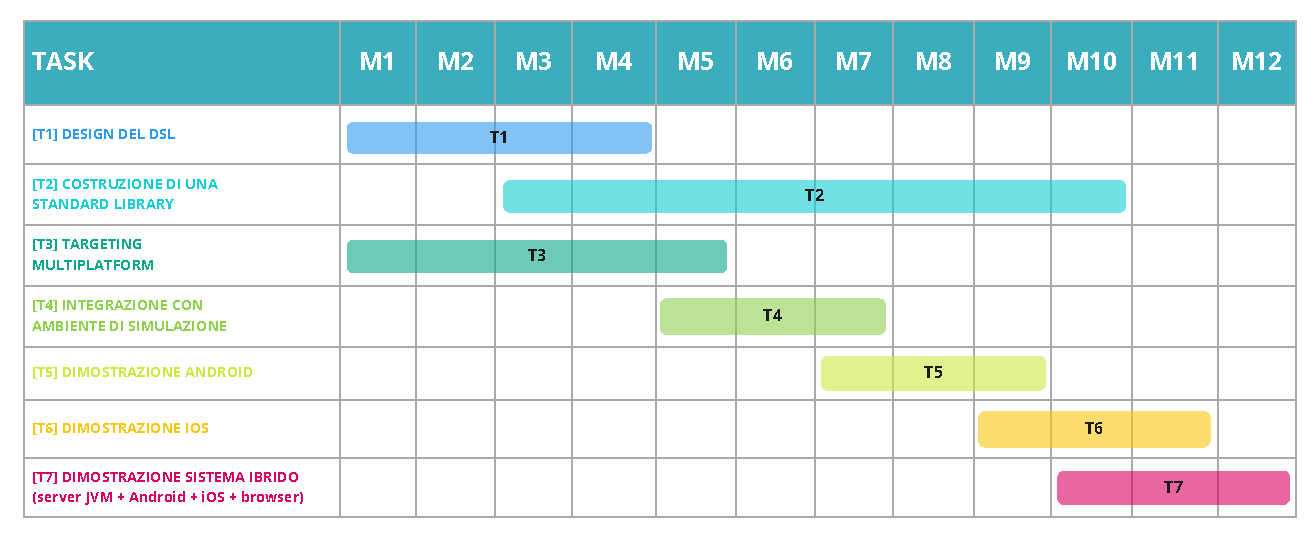
\includegraphics[width=\textwidth]{images/collektive_timeline}
    \caption{Timeline indicativa del progetto.}
    \label{fig:timeline}
\end{figure}

\subsection{Design del DSL [Task T1]}\label{subsec:t1}

\paragraph{DSL}
Per prima cosa è servito capire quali fossero effettivamente i costrutti necessari da inserire all'interno del DSL di \ck{}\footnote{
    Repository con codice open source visitabile al seguente link \url{https://github.com/Collektive/collektive}.
}.
%
Tra i vari approcci proposti per l'implementazione del \ac{FC}, è stato scelto di utilizzare \ac{xc}~\cite{AudritoCDSV24}.
%
\ac{xc} è un linguaggio di programmazione sperimentale per lo sviluppo di sistemi distribuiti omogenei che segue le astrazioni
    di \ac{AC}.

Astraendo da concorrenza, perdita di messaggi, protocollo di comunicazione di rete e fallimenti dei nodi,
    \ac{xc} permette di definire un modello di calcolo distribuito che si basa su un insieme di regole di trasformazione
    che operano sui campi computazionali,
    rivelandosi un modello di calcolo ideale per il progetto.

\ac{xc} è basato su una primitiva di comunicazione che permette di scambiare messaggi tra dispositivi e mantenere al contempo uno stato --\emph{exchange}--,
che sussume tutte le primitive di comunicazione del \ac{FC},
consentendo di implementare le altre primitive in modo derivato.
%
A partire dall'implementazione di \texttt{exchanging}, è stato possibile implementare le altre primitive di comunicazione del \ac{FC},
di seguito riassunte:
\begin{itemize}
    \item \texttt{exchanging}: implementa lo scambio di messaggi personalizzati con stato tra dispositivi ``vicini'',
    restituendo al programma un campo computazionale che rappresenta lo stato del proprio intorno;
    \item \texttt{exchange}: versione semplificata di \texttt{exchanging} che restituisce il medesimo campo utilizzato
    per determinare che informazione inviare ai vicini;
    \item \texttt{sharing}: implementato in termini di \texttt{exchange}, permette di condividere un valore ai vicini indistintamente
    dal destinatario, restituendo al programma un valore diverso da quello condiviso;
    \item \texttt{share}: come \texttt{sharing}, ma restituisce al programma il valore che è stato condiviso con i vicini;
    \item \texttt{repeating}: costrutto del \ac{FC} che permette di modellare l'evoluzione nel tempo dello stato del dispositivo.
    In quanto non è necessaria comunicazione con i vicini, non è stato implementato in termini di \texttt{exchange}.
    Restituisce al programma un valore diverso rispetto a quello su cui si effettuano le operazioni;
    \item \texttt{repeat}: \texttt{repeating}, ma restituisce al programma il valore su cui vengono effettuati i calcoli;
    \item \texttt{neighboring}: costrutto del \ac{FC} che permette di accedere ai valori dei vicini e inviare loro informazioni,
    permettendo così di modellare l'evoluzione dell'informazione nello spazio.
    Implementato sia in termini di \texttt{exchanging} che non, con differenze in termini di performance.
\end{itemize}

\paragraph{Compiler Plugin}

La comunicazione fra dispositivi in \ac{AC} è fondata sul concetto di ``allineamento''.
%
La semantica del \ac{FC} è definita compositiva ed i messaggi scambiati tra vicini vengono automaticamente abbinati
    allo stesso costrutto del programma, determinato da un processo chiamato allineamento.
%
Ogni costrutto genera un ``field'', un campo computazionale sul quale vengono eseguiti i calcoli, che viene
associato ad un ``path'' di esecuzione e successivamente inviato ai vicini.

Il meccanismo di allineamento assicura che ogni sotto-programma di un dispositivo sia abbinato al corrispondente dei vicini,
    seguendo un percorso identico nell'albero di valutazione,
    permettendo così di far comunicare i dispositivi allineati tra di loro.

Alcuni linguaggi che implementano la semantica del \ac{FC}, gestiscono l'allineamento in maniera esplicita (come nel linguaggio FCPP~\cite{fcpp}),
cioè richiedono che l'utente definisca esplicitamente le chiamate a funzione per eseguire l'allineamento,
rendendo il codice più verboso e meno trasparente,
altri invece non supportano la reificazione dei field, come in ScaFi~\cite{scafi}.

\ck{} si propone di gestire l'allineamento in modo trasparente e automatico, mantenendo la reificazione dei field,
attraverso l'estensione del compilatore di Kotlin tramite un plugin.
%
Il plugin del compilatore implementato si occupa di annotare le funzioni visitate durante la valutazione del programma,
in modo da poter creare un path di esecuzione che permetta di allineare i dispositivi tra di loro, con l'unica
responsabilità dell'utente di importare la dipendenza del plugin nel proprio progetto.

\subsection{Costruzione di una standard library [Task T2]}\label{subsec:task-t2-[costruzione-di-una-standard-library]}

Le primitive esposte da \ac{xc}, sebbene dimostratamente universali,
sono, all'atto pratico dell'ingegneria dei sistemi software,
di basso livello e non facilmente utilizzabili direttamente.
%
Di conseguenza, sfruttando la componibilità delle primitive di \ac{FC},
si vuole costruire una libreria standard di comportamenti auto-organizzanti,
che sarà (grazie alla composizione funzionale) riutilizzabile per costruire comportamenti più complessi.

La selezione delle funzionalità da inserire nella standard library
è ancora in corso,
e l'approccio scelto è di tipo bottom-up:
a partire dalla realizzazione di casi di studio,
vengono identificati i blocchi che vengono utilizzati più frequentemente,
la loro generalizzazione andrà a comporre la libreria standard.

Come primo passo,
è stata implementata una generalizzazione di un algoritmo noto in letteratura,
chiamato \ac{vmc}~\cite{ZahadatHS17},
applicando un approccio basato su \ac{AC}, utilizzando il \ac{dsl} \ck{}.
%
\ac{vmc} permette di modellare la crescita di strutture artificiali nel tempo ispirandosi alla morfogenesi delle piante.
%
L'algoritmo si basa su un modello di distribuzione delle risorse in strutture ad albero,
    dove i rami competono per le risorse per crescere, in base al successo ottenuto come input da sensori nell'ambiente.

Implementando l'algoritmo con \ck{},
è stato possibile identificare le funzionalità chiave da cui partire per costruire la standard library.
%
In particolare,
sono stati identificati alcuni metodi di riduzione dei campi computazionali, come ad esempio la somma tra field
e funzioni che permettano di filtrare il field in base a condizioni passate come parametri.
%
Inoltre, sono stati utilizzati i blocchi di base presentati in~\cite{TOMACS2018}:
gradiente e gradient-cast, converge-cast, e sparse choice (processo di leader election).
%
Quest'ultimo è stato implementato come bounded election~\cite{PianiniCV22},
recentemente dimostrato essere auto-stabilizzante~\cite{Dijkstra74}.

Dal lavoro,
ottenuto con lo sviluppo dell'algoritmo,
svolto con la collaborazione del gruppo di ricerca ospitante,
è stato possibile realizzare un articolo scientifico alla conferenza
``\emph{Autonomic Computing and Self-Organizing Systems}'' (ACSOS) 2024\footnote{\url{https://2024.acsos.org}}
(il manoscritto è attualmente in revisione).

\subsection{Modifica al programma: Task T4}\label{subsec:modifica-al-programma:-task-t4}

Per poter validare il lavoro svolto, è stata necessaria l'integrazione con un simulatore,
    per controllare la correttezza del sistema e comprenderne il comportamento in scenari diversi.
%
\ck{} è stato quindi rudimentalmente integrato con un ambiente di simulazione noto,
anticipando di qualche mese l'inizio del task T4, ovvero l'integrazione con un ambiente di simulazione.
%
Come ambiente di simulazione, è stato scelto \emph{Alchemist}~\cite{PianiniJOS2013},
un meta-simulatore per pervasive computing e sistemi distribuiti,
basato su astrazioni generali che possono essere mappate a casi d'uso specifici.
%
Il simulatore è sviluppato e mantenuto dal gruppo di ricerca ospitante,
che ha fornito supporto per l'integrazione.
%
Data l'integrazione con \emph{Alchemist}, è stato possibile creare alcuni esperimenti nell'ambito di \ac{vmc},
    sempre presentati ad ACSOS 2024, che hanno permesso di validare il lavoro svolto \footnote{
    Gli esperimenti sono open source ed è possibile visionarli al seguente link \url{https://github.com/angelacorte/vmc-experiments}.
}.

\subsection{Targeting multiplatform [Task T3]}\label{subsec:task-t3-[targeting-multiplatform]}
Per quanto riguarda il targeting delle varie piattaforme,
    sono stati implementati test che verificano il funzionamento su più piattaforme.
%
I test vengono eseguiti automaticamente ad ogni push sul repository, grazie all'integrazione con GitHub Actions in modalità \ac{cicd}.

Il \ac{dsl} è dunque testato con esiti positivi su \ac{JVM}, Javascript, nativo ed emulatore di iOS, watchOS e tvOS.
%
Al momento non sono ancora presenti test specifici per Android,
per i quali, al momento,
si fa affidamento su quelli \ac{JVM}
(Android è in grado di importare ed eseguire software scritto per \ac{JVM}).

\section{Prossimi obiettivi}\label{sec:prossimi-obiettivi}

%completamento t1 t3
%implementazione standard library in contrapposizione a quella di protelis -francia
%ulteriori sviluppi di t4
%allineamento debug-friendly
%investigare integrazione con pulverization

Come obiettivi per i prossimi tre mesi di lavoro, ovvero nella figura~\ref{fig:timeline} tra M6 e M7,
    si prevede di completare il task T1, ovvero la progettazione del \ac{dsl},
    ed il task T3, ovvero il targeting multiplatform,
    aspirando all'effettivo testing del \ac{dsl} su Android e piattaforme iOS fisiche.
%
Gli sviluppi dell'integrazione con l'ambiente di simulazione (task T4) e della standard library (task T2) verranno portati
avanti, con l'obiettivo di implementare funzionalità come, ad esempio, funzioni di broadcast,
calcolo di un gradiente all'interno di una specifica regione e l'individuazione di canali in corrispondenza di percorsi minimi tra due punti.

Durante lo sviluppo della generalizzazione del modello \ac{vmc}, è stato indivuduato un problema di chiarezza in fase di debugging
inerente al path generato dal plugin del compilatore.
%
La figura~\ref{fig:alignment} mostra vari utilizzi innestati di funzioni lambda, ognuna delle quali ha come path di esecuzione
``$\$1$'', rendendo poco chiaro il comportamento del programma.
%
Il path creato dal plugin del compilatore, inerente all'allineamento di varie funzioni lambda innestate, non è facilmente comprensibile
agli occhi di qualcuno che non conosce il funzionamento interno del plugin stesso.
\begin{figure}
    \centering
    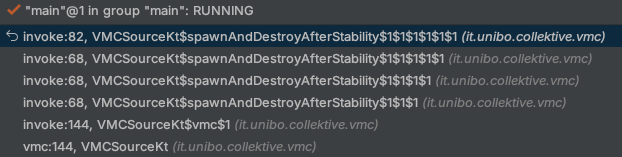
\includegraphics[width=\textwidth]{images/alignment}
    \caption{Esempio di path generato dal plugin del compilatore visto in fase di debugging.}
    \label{fig:alignment}
\end{figure}

Per risolvere questo problema, si prevede di implementare un meccanismo di allineamento più debug-friendly,
    che permetta di visualizzare in modo chiaro il comportamento dei dispositivi durante l'esecuzione del programma.

Come attuale lavoro in svolgimento c'è anche la stesura di un altro articolo, che verrà presentato alla conferenza
    ``\emph{Distributed Simulation and Real Time Applications}'' (DS-RT) 2024~\footnote{\url{http://ds-rt.com/2024/}},
    per il quale verranno sviluppate simulazioni di programmi implementati con \ck{} in un ambiente di simulazione distribuito.

Infine, si prevede di collaborare ulteriormente col gruppo di ricerca che ospita l'attività corrente,
dove sono in corso
    ricerche sull'approccio a ``polverizzazione''~\cite{fi12110203},
    utilizzato per suddividere il comportamento complessivo del sistema
in piccoli pezzi il cui deployment può essere determinato a runtime.
%
Questa collaborazione potrebbe portare a una posticipazione dei task inerenti alle demo (T6, T7, T8), ma permetterebbe di sviluppare
    un approccio più generale e flessibile per la programmazione di dispositivi eterogenei nell'edge-cloud continuum.

%%%%%%%%%%%%%%%%%%%%end%%%%%%%%%%%%%%%%%%%%

% add more ....

\bibliographystyle{plain}
\bibliography{bibliography}

\end{document}